\chapter{Results}
\section{Carotid Segmentation from MRA-TOF}
The measures described in Section~\ref{sec:carotid} significantly improved carotid segmentation by effectively excluding brain lesions and undesired venous structures.
As illustrated in Figure~\ref{fig:seg_compare}, the cuboid mask plays a crucial role in this process.
Because no ground truth segmentation is available, visual inspection was used to evaluate the results, which showed that lesions and venous structures were rarely selected by the algorithm.
However, the algorithm acted overly conservative at times. It inadvertently excluded the periphery of the larger vessels or completely excluded the narrow ones.
\begin{figure}[h]
	\centering
	\begin{subfigure}{0.45\textwidth}
		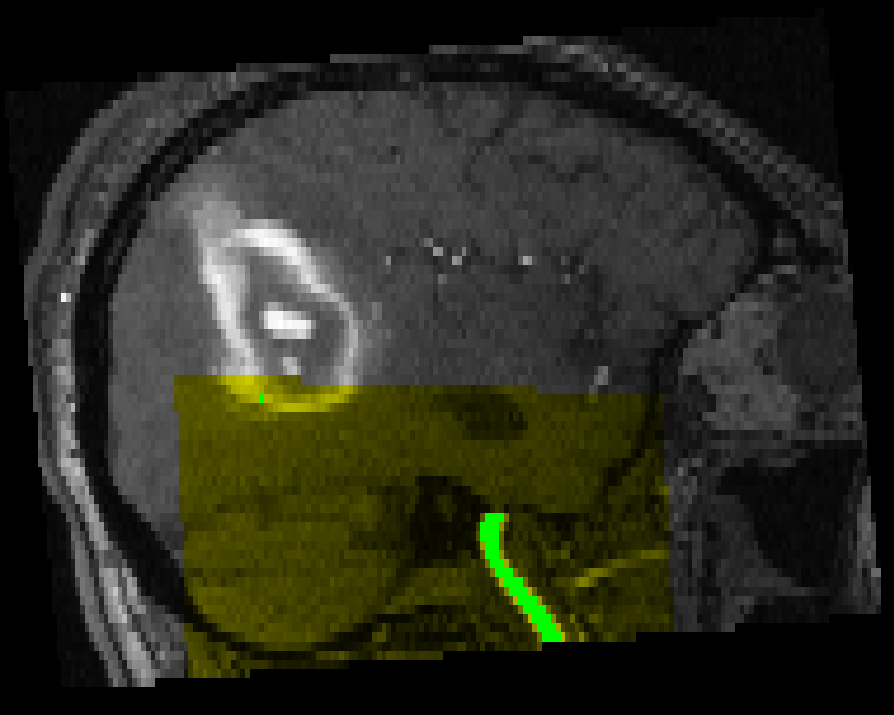
\includegraphics[width=\textwidth]{figures/molgu07704_bbox.png}
		\caption{}
		\label{subfig:seg_bbox}
	\end{subfigure}
	\begin{subfigure}{0.45\textwidth}
		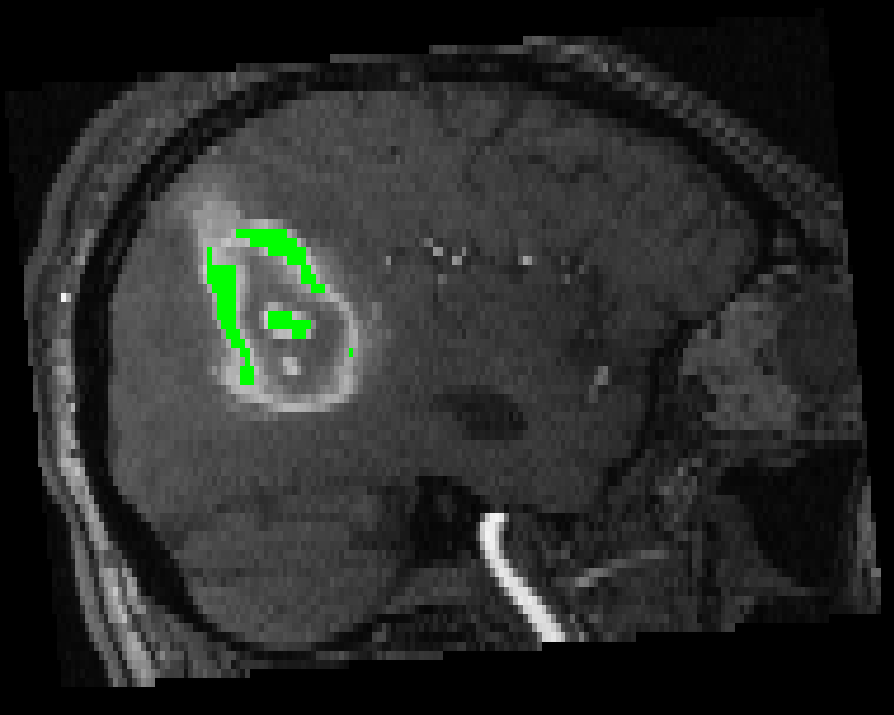
\includegraphics[width=\textwidth]{figures/molgu07704_nobbox.png}
		\caption{}
		\label{subfig:seg_nobbox}
	\end{subfigure}
	\caption{Comparison of carotid segmentation (green) with (a) and without (b) a cuboid mask (yellow). In the absence of the cuboid mask, the segmentation algorithm fails to capture the carotid and instead incorrectly identifies the brain lesion}
	\label{fig:seg_compare}
\end{figure}
\section{IDIF}
IDIF estimation was performed using both the Bayesian GTM (BGTM) and conventional GTM PVC methods.
Figure~\ref{fig:ifs} compares the two methods for one of the best- and worst-performing subjects.
In the well-performing subject, BGTM significantly outperforms GTM; however, in the poorly performing case, BGTM falls short of GTM.
The average mean absolute error of the cAUC curves across the dataset was 14,202 for BGTM and 33,764 for GTM (Figure~\ref{subfig:cauc_boxplot}).

\begin{figure}[h]
	\centering
	\begin{subfigure}[b]{0.322\textwidth}
		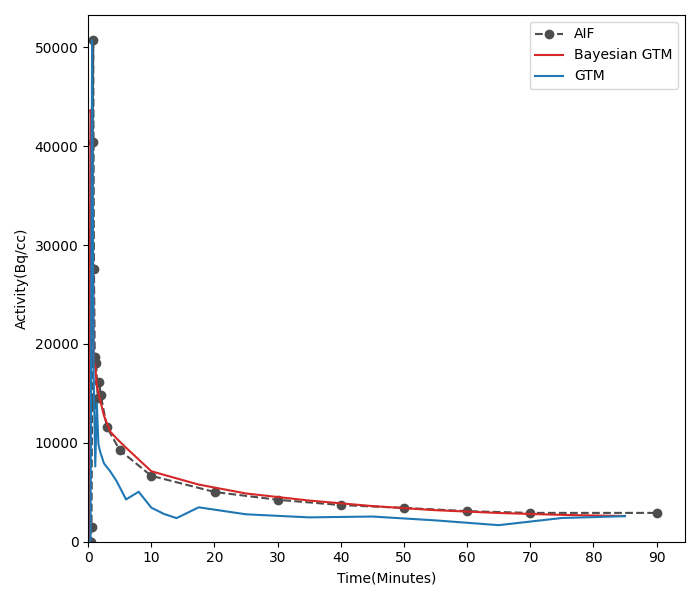
\includegraphics[width=\textwidth]{figures/MOLGU07704_1_if_comparison.png}
		\caption{}
		\label{subfig:good_if_compare}
	\end{subfigure}
	\begin{subfigure}[b]{0.322\textwidth}
		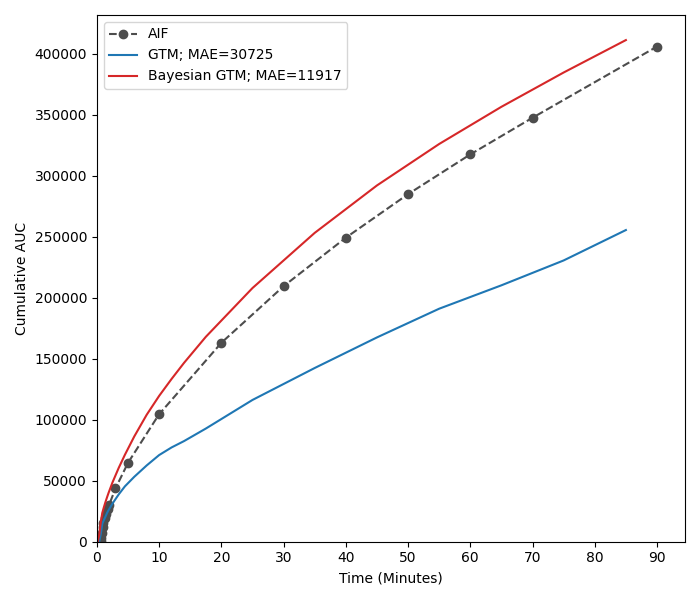
\includegraphics[width=\textwidth]{figures/MOLGU07704_1_trap.png}
		\caption{}
		\label{subfig:good_trap_compare}
	\end{subfigure}
	\begin{subfigure}[b]{0.322\textwidth}
		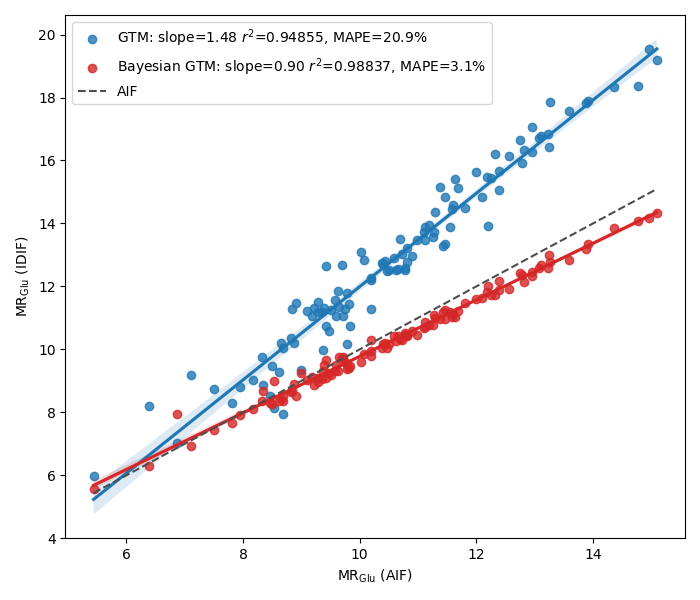
\includegraphics[width=\textwidth]{figures/MOLGU07704_1_cmrglu.png}
		\caption{}
		\label{fig:good_cmrglu}
	\end{subfigure}
	\begin{subfigure}[b]{0.322\textwidth}
		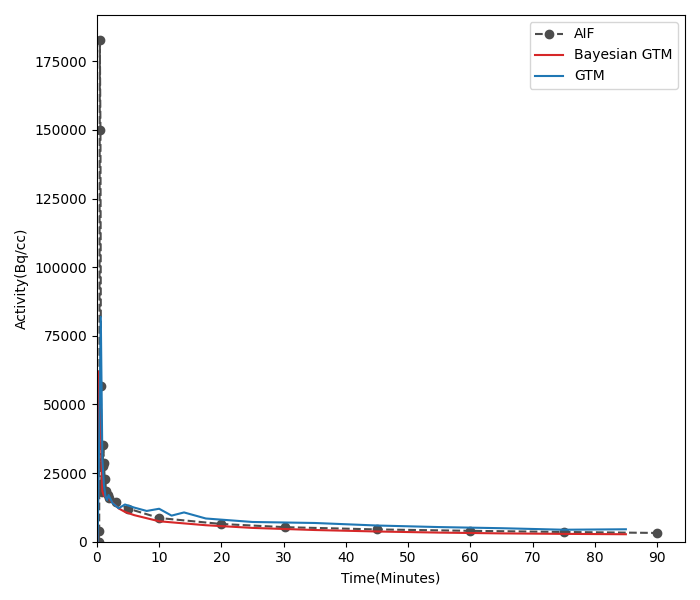
\includegraphics[width=\textwidth]{figures/CM10250_1_if_comparison.png}
		\caption{}
		\label{subfig:bad_if_compare}
	\end{subfigure}
	\begin{subfigure}[b]{0.322\textwidth}
		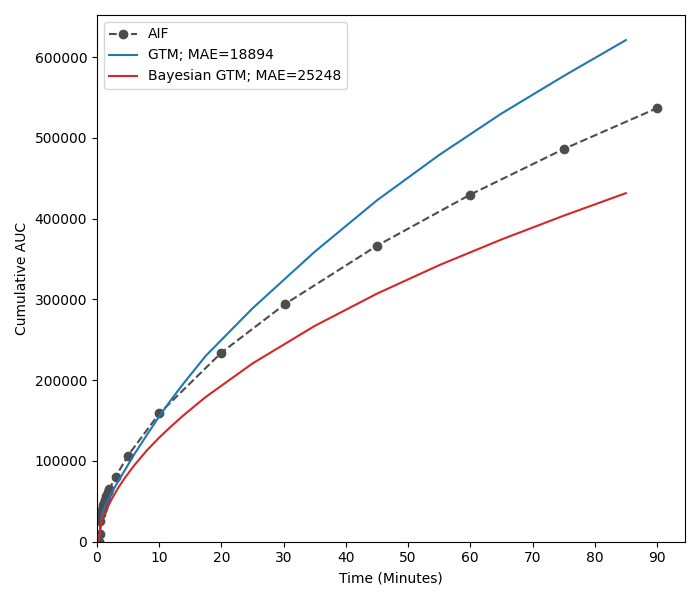
\includegraphics[width=\textwidth]{figures/CM10250_1_trap.png}
		\caption{}
		\label{subfig:bad_trap_compare}
	\end{subfigure}
	\begin{subfigure}[b]{0.322\textwidth}
		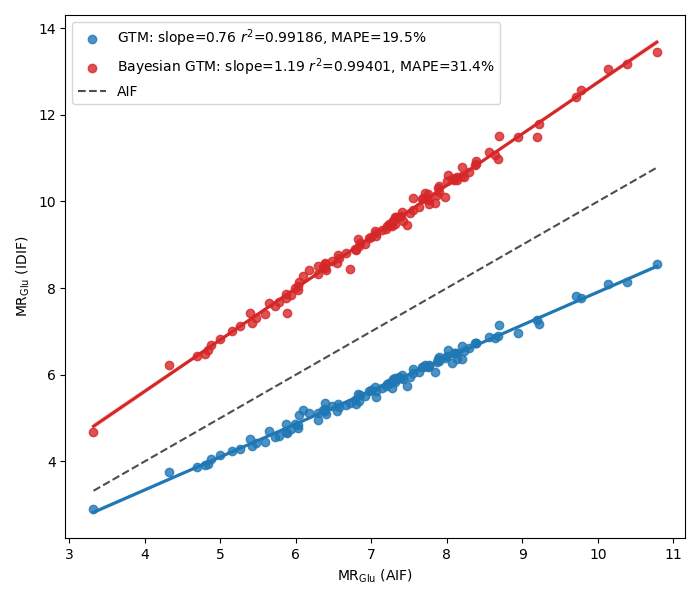
\includegraphics[width=\textwidth]{figures/CM10250_1_cmrglu.png}
		\caption{}
		\label{fig:bad_cmrglu}
	\end{subfigure}
	\caption{Comparison of the IFs (a,d), cumulative AUC curves (b,e), and $\mrglu$ regression lines (c,f) for one of the best-(top row) and worst-performingr(bottom row) subjects}
	\label{fig:ifs}
\end{figure}

ROI-based quantification was carried out using both IDIF methods, with BGTM yielding significantly better performance.
Specifically, the BGTM and GTM methods achieved an average \(\mrglu\) mean absolute percentage error (MAPE) of 14.1\% and 33\%, respectively (Figure~\ref{subfig:mape_boxplot}), and an average \(\mrglu\) MAE of 1.42 and 3.5.
In addition, the MAE for the coefficient of determination (\(R^2\)) and the regression slope (\(S\)) were 0.004 and 0.14 for BGTM, compared to 0.030 and 0.304 for GTM, respectively.

\begin{figure}
	\centering
	\begin{subfigure}[b]{0.45\textwidth}
		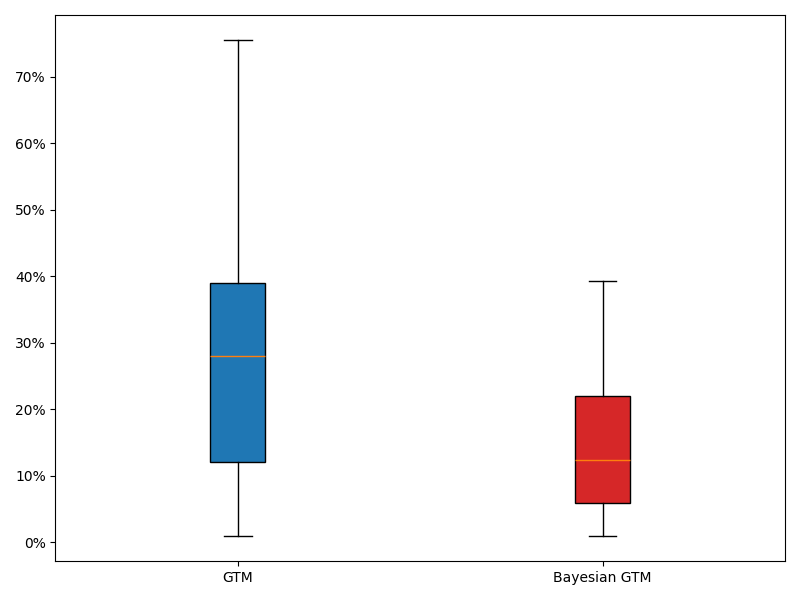
\includegraphics[width=\textwidth]{figures/quantification_mape_fitk3_boxplot.png}
		\caption{\(\mrglu\) MAPE Boxplot}
		\label{subfig:mape_boxplot}
	\end{subfigure}
	\begin{subfigure}[b]{0.45\textwidth}
		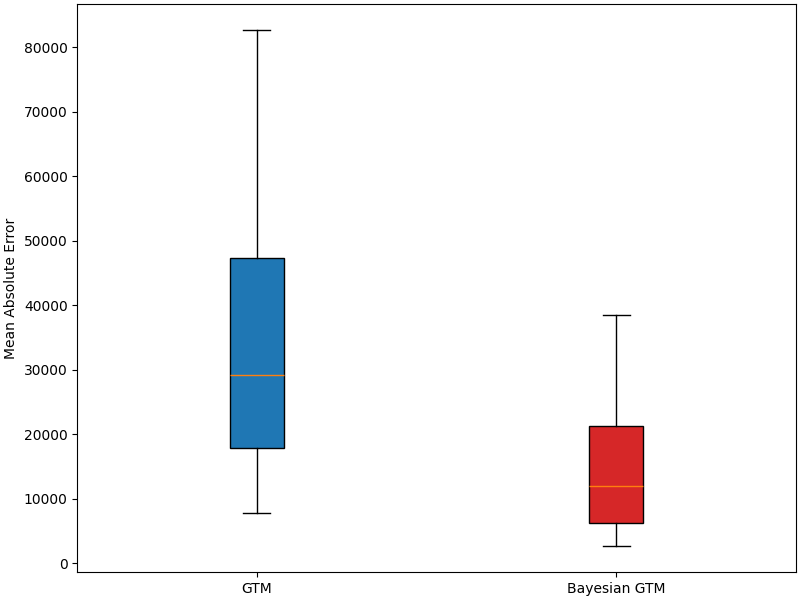
\includegraphics[width=\textwidth]{figures/curve_errors_boxplots.png}
		\caption{cAUC MAE Boxplot}
		\label{subfig:cauc_boxplot}
	\end{subfigure}
	\caption{Boxplot of curve and quantification errors}
	\label{fig:boxplots}
\end{figure}

\begin{table}[b]
	\centering
	\begin{tabular}{l|cc|cc|cc}
		\toprule
		\multirow{3}{*}{\textbf{Metric}} & \multicolumn{2}{c|}{\textbf{BGTM}} & \multicolumn{2}{c}{\textbf{GTM}} & \multicolumn{2}{c}{\textbf{Paired T-Test}}                                                 \\
		\cmidrule(lr){2-3} \cmidrule(lr){4-5} \cmidrule(lr){6-7}
		                                 & \(\mu\)                            & \(\sigma\)                       & \(\mu\)                                    & \(\sigma\) & T-Value & P-Value                \\
		\midrule
		IF cAUC MAE                      & 14,202                             & 9,190                            & 33,764                                     & 21,212     & 7.44    & \(7.2\times 10^{-10}\) \\
		$\mrglu$ MAPE (\%)               & 14.1                               & 10.1                             & 33.0                                       & 31.5       & 4.32    & \(6.5\times 10^{-5}\)  \\
		$\mrglu$ MAE                     & 1.42                               & 1.07                             & 3.50                                       & 3.38       & 4.41    & \(4.8\times 10^{-5}\)  \\
		$\mrglu$ \(R^2\) MAE             & 0.004                              & 0.006                            & 0.030                                      & 0.132      & 1.45    & \(1.5\times 10^{-1}\)  \\
		$\mrglu$ Slope MAE               & 0.14                               & 0.109                            & 0.304                                      & 0.230      & 4.73    & \(1.6\times 10^{-5}\)  \\
		\bottomrule
	\end{tabular}
	\caption{Summary of performance metrics for BGTM and GTM methods and their paired t-test.
		% $\mu$ is the average and $\sigma$ is the standard deviation
	}
	\label{tab:metrics}
\end{table}

A paired t-test was conducted to compare the performance of BGTM and GTM across previously mentioned metrics.
The results, summarized in Table~\ref{tab:metrics}, indicate that BGTM significantly outperforms GTM in cAUC MAE(\( t = 7.44 \), \( p = 7.2 \times 10^{-10} \)), $\mrglu$ MAPE (\( t = 4.32 \), \( p = 6.5 \times 10^{-5} \)), $\mrglu$ MAE (\( t = 4.41 \), \( p = 4.8 \times 10^{-5} \)), and $\mrglu$ Slope MAE (\( t = 4.73 \), \( p = 1.6 \times 10^{-5} \)), demonstrating the effectiveness of the proposed method.
However, no significant difference was observed in $\mrglu$ \(R^2\) MAE (\( t = 1.45 \), \( p = 0.15 \)).

As illustrated in Figure~\ref{fig:corr_mat}, there is a strong correlation between the cAUC MAE and the quantification errors suggesting cAUC as a reliable intermediate metric.

\begin{figure}[h]
	\centering
	\begin{subfigure}{0.45\textwidth}
		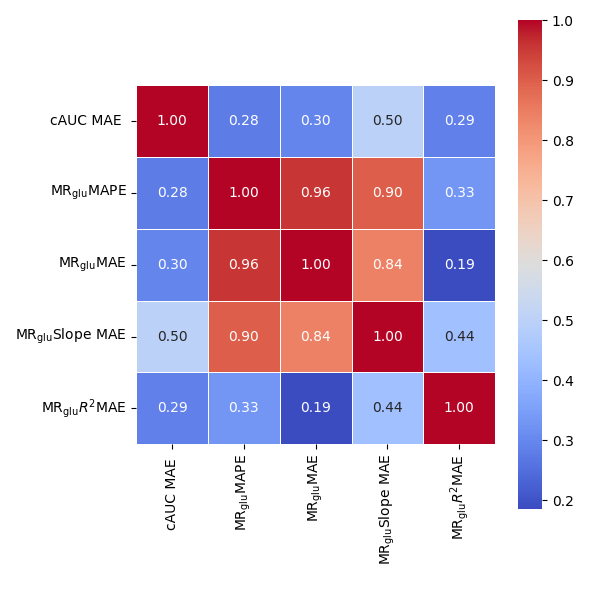
\includegraphics[width=\textwidth]{figures/corr_gtm.png}
		\caption{GTM}
		\label{subfig:corr_gtm}
	\end{subfigure}
	\begin{subfigure}{0.45\textwidth}
		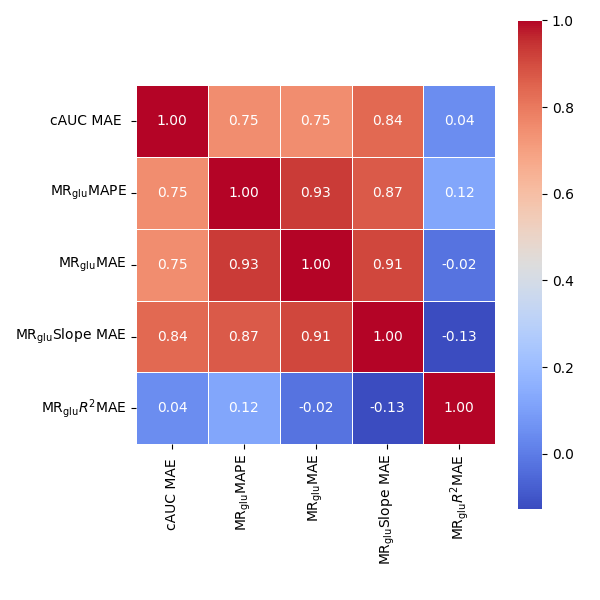
\includegraphics[width=\textwidth]{figures/corr_bgtm.png}
		\caption{Bayesian GTM}
		\label{subfig:corr_bgtm}
	\end{subfigure}
	\caption{Correlation matrix of different metrics for Bayesian GTM and GTM methods}
	\label{fig:corr_mat}
\end{figure}



